\subsection{Planning second half}
% 1 page
To get the project back on track we need an overview of the remaining parts of the project, an estimate of how much time we have left, and a carefully structured plan on the order of the activities we have left to do.\\
We have divided the planning into four parts.

We start by determining the development methods we want to use. We give a brief introduction to each method, and explain how we applied it to help the project back on track.

After this we will select the estimation method(s) we will use. The estimation methods should help us make accurate estimations and based on these, decisions. Through correct decisions based on close to correct estimates, the estimation methods will help us meet the deadline.

When we have found how much time we need, we need to find out how much time we have available. If we have less time than required, we will need to cut down on functionality. As learned in the first part of the project, no good results are yielded from trying to squeeze more functionality into the schedule than it realistically has room for.
To get an overview of our time we will select a couple of planning methods. The methods will be explained, and our usage will be analyzed.

As the last, but possibly the most important part, we look into how our project recovery has affected the quality. Less time to do roughly the same work must have some effect on the quality, since the time, cost, and quality of a product are constrained by each other (see figure \ref{fig:timeCostsQuality})\cite[p. 191]{PM}. In the final part we will analyze this aspect of our project.

\begin{figure}[t]
  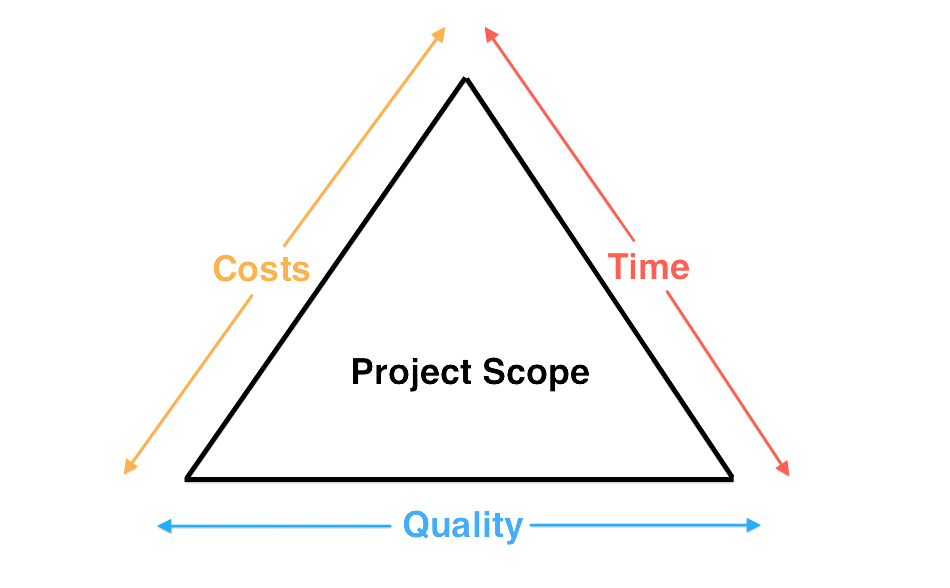
\includegraphics[width=\textwidth]{illustrations/timeCostsQuality}
  \caption{The triple constraint: When the requirements to costs, timescale, or quality change, the resources assigned to the other aspects must change accordingly as well.}
  \label{fig:timeCostsQuality}
\end{figure}
